\section{Experimental Evaluation}
\label{sec:experiments}

The experiments ask four questions. Do controlled relations improve intent-oriented features over an identical reconstruction-only model? Do these gains remain when reconstruction and activity are measured? Are the learned features stable and interpretable across held-out locales? Finally, do the conclusions transfer across sparse widths, datasets, and model families? Appendix~\ref{app:protocol} contains the complete protocol and configuration.

\subsection{Experimental design}

\paragraph{Models and data.}
The main experiment uses masked-mean hidden-state-8 activations from Gemma~2~2B \citep{gemmateam2024gemma2} on MASSIVE \citep{fitzgerald2023massive}. Training contains 10,343 semantic IDs from 49 locales; validation contains 1,149 disjoint IDs. The final test set contains 2,968 untouched IDs, each observed in Arabic and Chinese. Transfer experiments use MTOP \citep{li2021mtop} and Pythia-160M \citep{biderman2023pythia}.

\paragraph{Fair comparisons.}
We compare raw $H$, global BatchTopK, the exact blockwise reconstruction control, Matryoshka SAE reconstruction, one-sided supervision, and a validation-selected triplet loss \citep{schroff2015facenet}. Learned comparisons share their inputs, dictionary capacity, activity, initialization, batches, optimizer, epochs, and paired seeds. Thus the blockwise control differs from our model only in the relational objective.

\paragraph{What a successful route should do.}
A useful $z_C$ feature should identify an intent, activate consistently for its translations, and reveal less locale information. We measure these properties with intent concept AUC, Arabic--Chinese activation correlation, and a locale probe. Intent- and locale-oriented feature fractions show which factor dominates the active dictionary. The reciprocal diagnostics ask whether $z_S$ retains locale while suppressing intent.

Intent concept AUC is the mean one-vs-rest held-out AUC \citep{fawcett2006roc} of one validation-selected coordinate per intent. Stability is the mean Pearson correlation \citep{pearson1895regression} between paired Arabic and Chinese activations. Balanced logistic probes \citep{cox1958regression} measure locale in $z_C$ and locale or intent in $z_S$. We report reconstruction as fraction of variance explained (FVE) and sparsity as the observed number of active features.

Every method uses the same feature-selection split, probe split, test split, and evaluator. Features are selected only on validation data, and all comparison tables report mean $\pm$ standard deviation over three paired seeds. Appendix~\ref{app:protocol} defines feature activity, orientation, probe selection, and bootstrap estimation.

\paragraph{Validation before testing.}
Validation selects the reciprocal binary objective and triplet margin $m=.2$ from $\{.1,.2,.4\}$. The Arabic--Chinese test activations are then evaluated once. No test result selects a model, feature, intent, or displayed example.

\subsection{Controlled relations reorganize the routes}

\begin{table*}[t]
\centering
\caption{MASSIVE results on held-out Arabic and Chinese. Blockwise methods are evaluated on $z_C$ in the primary columns. Lower locale probe, locale-oriented fraction, and $z_S$ intent probe are better.}
\label{tab:factor-sae-test}
\resizebox{\textwidth}{!}{%
\begin{tabular}{lrrrrrrrr}
\toprule
Method & Intent AUC $\uparrow$ & Stability $\uparrow$ & Locale probe $\downarrow$ & Intent frac. $\uparrow$ & Locale frac. $\downarrow$ & $z_S$ locale $\uparrow$ & $z_S$ intent $\downarrow$ & FVE $\uparrow$ \\
\midrule
Raw $H$ & .7703 & .3013 & .9997 & .1159 & .7409 & -- & -- & -- \\
BatchTopK SAE & $.7940\pm.0014$ & $.1278\pm.0011$ & $.9871\pm.0048$ & $.4579\pm.0026$ & $.4723\pm.0030$ & -- & -- & $.6618\pm.0017$ \\
Blockwise control & $.7007\pm.0109$ & $.1501\pm.0080$ & $.9665\pm.0106$ & $.4830\pm.0122$ & $.4465\pm.0122$ & $.9878\pm.0014$ & $.4798\pm.0151$ & $.6627\pm.0002$ \\
Matryoshka SAE & $.8352\pm.0150$ & $.1385\pm.0017$ & $.9821\pm.0009$ & $.4686\pm.0018$ & $.4652\pm.0033$ & -- & -- & $.6482\pm.0014$ \\
One-sided factor SAE & $\mathbf{.9165\pm.0083}$ & $.1813\pm.0061$ & $.8969\pm.0143$ & $.6923\pm.0198$ & $.2427\pm.0163$ & $.9861\pm.0029$ & $.4679\pm.0004$ & $.6415\pm.0015$ \\
\textbf{Reciprocal factor SAE (ours)} & $.9124\pm.0027$ & $\mathbf{.2248\pm.0035}$ & $\mathbf{.8944\pm.0034}$ & $\mathbf{.7864\pm.0144}$ & $\mathbf{.1646\pm.0065}$ & $\mathbf{.9925\pm.0008}$ & $.3892\pm.0079$ & $.6098\pm.0011$ \\
Triplet, $m=.2$ & $.9063\pm.0190$ & $.1983\pm.0029$ & $.9096\pm.0049$ & $.7274\pm.0013$ & $.2043\pm.0011$ & $.9916\pm.0029$ & $\mathbf{.3818\pm.0171}$ & $\mathbf{.6427\pm.0012}$ \\
\bottomrule
\end{tabular}%
}
\end{table*}

Controlled relations reorganize both routes in the intended direction. Against the exact blockwise control, our $z_C$ raises intent AUC from .7007 to .9124 and stability from .1501 to .2248. Its intent-oriented feature fraction rises from .4830 to .7864, while its locale-oriented fraction falls from .4465 to .1646. The reciprocal $z_S$ route reaches .9925 locale accuracy and reduces intent leakage from .4798 to .3892. Because the control removes only the relational losses, these changes isolate relational supervision.

The same conclusion holds against the standard sparse alternatives. Relative to global BatchTopK, intent AUC increases by .1185 and stability by .0970; relative to Matryoshka, the gains are .0772 and .0863. The complete-route intent probe remains close to global BatchTopK (.4625 versus .4680), indicating that stronger organization in $z_C$ does not remove intent from the joint sparse code.

Raw $H$ is a dense reference, not a sparse baseline. Locale is almost perfectly decoded from it (.9997), and 74.1\% of its coordinates are locale-oriented. In contrast, the learned $z_C$ is sparse and overcomplete, with 78.6\% intent-oriented and 16.5\% locale-oriented active features. The result is therefore a change in feature organization, not simply the presence of intent somewhere in the representation.

\subsection{Reconstruction and activity}

The factor gains are obtained at matched sparse activity with a moderate reconstruction trade-off. All models train at mean $L_0=64$, and their frozen thresholds produce similar held-out activity: $104.46\pm.07$ for ours, $105.99\pm.81$ for the exact control, and $107.16\pm.91$ for global BatchTopK. Reconstruction FVE is .6098 for ours and .6627 for the exact control, an 8.0\% relative difference.

Held-out $L_0$ exceeds the training budget because test examples use thresholds calibrated on seen locales rather than a newly computed test-batch budget. Since ours and the controls have nearly identical held-out activity, the AUC and stability gains cannot be explained by a larger test-time code. Appendix~\ref{app:protocol} gives the shared thresholding and reconstruction protocol.

\subsection{Cross-locale feature consistency}

\begin{figure*}[t]
\centering
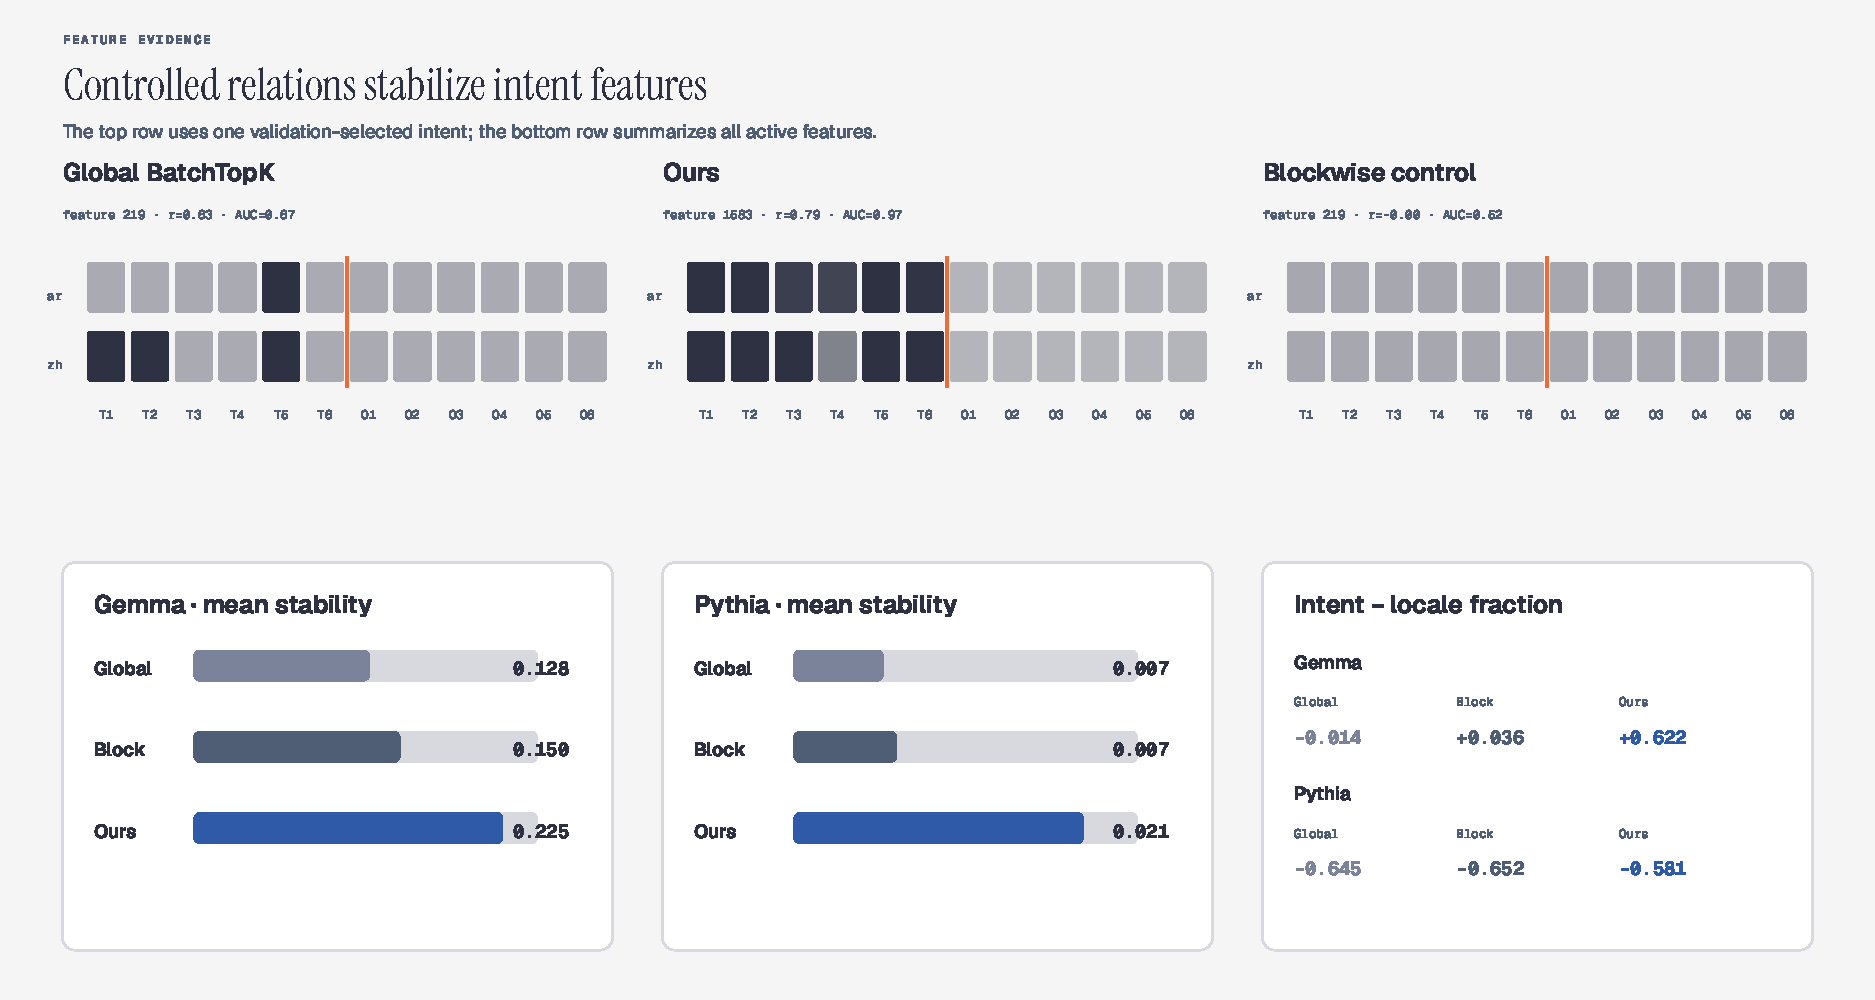
\includegraphics[width=\textwidth]{Figures/factor_sae_figure3_stability.pdf}
\caption{Controlled relations stabilize intent features. Top: each Gemma method selects its own feature for the same validation-selected intent; T1--T6 and O1--O6 are held-out target- and comparison-intent semantic IDs in Arabic and Chinese. Bottom: three-seed all-feature stability and intent-minus-locale orientation for Gemma and Pythia.}
\label{fig:factor-feature-stability}
\end{figure*}

Figure~\ref{fig:factor-feature-stability} shows what the aggregate stability gain looks like for one intent feature. The reciprocal feature responds similarly to Arabic and Chinese instances of its target intent, reaching held-out AUC .97 and stability .79. The blockwise-control feature for the same validation-selected intent reaches AUC .52 and approximately zero stability. The dictionary-wide averages give the same ordering for both Gemma (.2248 versus .1501) and Pythia (.0211 versus .0075).

Feature and intent selection use disjoint validation splits; held-out activations are never used to choose the example. Test labels only identify the six deterministically ordered target and comparison instances after selection. The complete selection rule appears in Appendix~\ref{app:protocol}.

\subsection{Intent-feature interpretability}

\begin{table*}[t]
\centering
\caption{Validation-selected intent features on held-out MASSIVE Arabic and Chinese. Purity and reliable coverage use 46 intents with at least 20 test semantic IDs; stability covers all 58 intents.}
\label{tab:factor-feature-interpretability}
\resizebox{.92\textwidth}{!}{%
\begin{tabular}{lrrrr}
\toprule
Method & Purity@20 $\uparrow$ & Reliable coverage $\uparrow$ & Selected stability $\uparrow$ & Top-ID overlap $\downarrow$ \\
\midrule
Global BatchTopK & $.653\pm.020$ & $.370\pm.022$ & $.457\pm.004$ & $.0025\pm.0005$ \\
Blockwise control & $.581\pm.068$ & $.341\pm.091$ & $.375\pm.040$ & $.0034\pm.0012$ \\
\textbf{Reciprocal factor SAE (ours)} & $\mathbf{.817\pm.012}$ & $\mathbf{.725\pm.045}$ & $\mathbf{.563\pm.003}$ & $\mathbf{.0022\pm.0001}$ \\
\bottomrule
\end{tabular}%
}
\end{table*}

The stable features are also more interpretable. Reciprocal supervision raises Purity@20 by .236 and reliable coverage by .384 over the exact blockwise control. Its near-zero top-ID overlap indicates that different intent features retrieve distinct examples rather than the same globally active utterances.

Purity ranks unique semantic IDs by the larger activation across their Arabic and Chinese translations. The calculation covers the 46 intents with at least 20 held-out IDs; reliable coverage is the fraction whose selected feature reaches at least .8 purity. Selected-feature stability covers all 58 intents.

The normalized locale entropy of our top activation sets is .633, close to global BatchTopK (.636), so high purity does not come from retrieving only one held-out locale. Appendix~\ref{app:feature-examples} provides the complete 58-intent catalogue and qualitative examples.

\begin{figure*}[t]
\centering
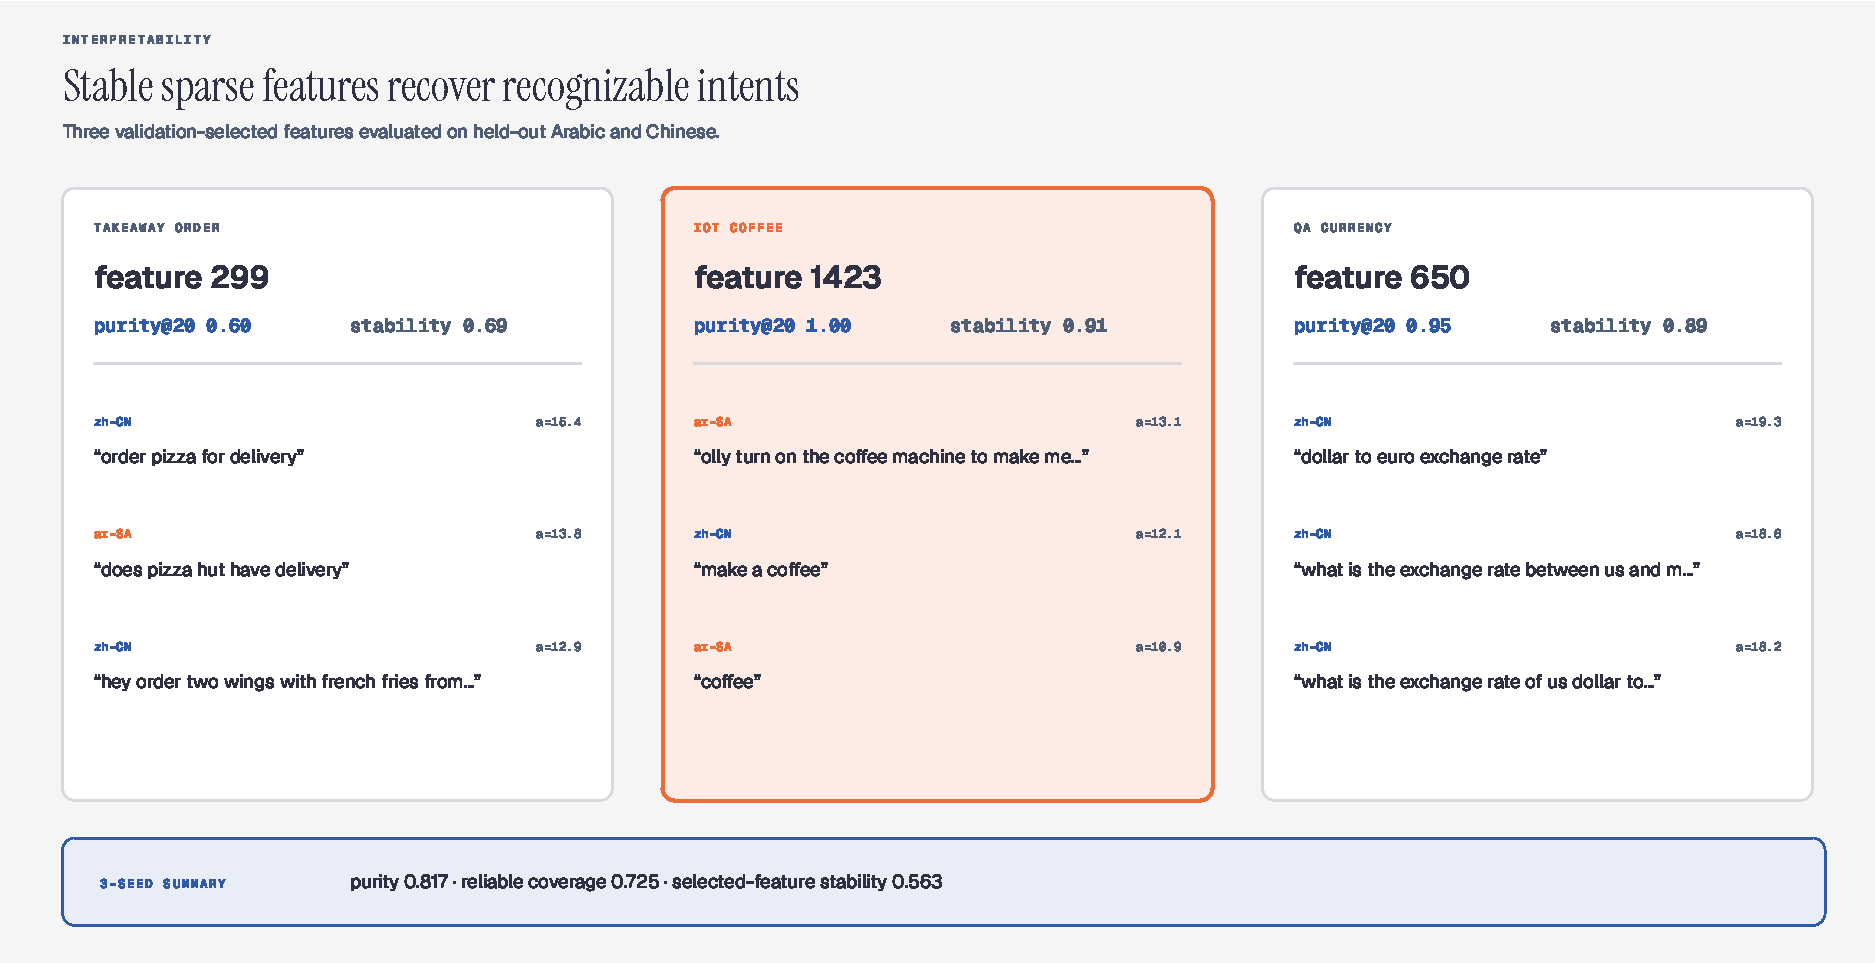
\includegraphics[width=\textwidth]{Figures/factor_sae_figure4_examples.pdf}
\caption{Validation-selected sparse features recover recognizable intent concepts on held-out Arabic and Chinese. The cards show representative high-activation examples for three intent features; selection uses validation data only, while purity and stability are measured on the held-out locales.}
\label{fig:factor-sae-examples}
\end{figure*}

The complete representative-seed catalogue contains all 58 intent features, including feature IDs, purity, stability, held-out AUC, and activity support (Appendix~\ref{app:feature-examples}). The machine-readable catalogue extends this evaluation to all three methods and seeds.

\subsection{Robustness, transfer, and ablations}

\begin{figure*}[t]
\centering
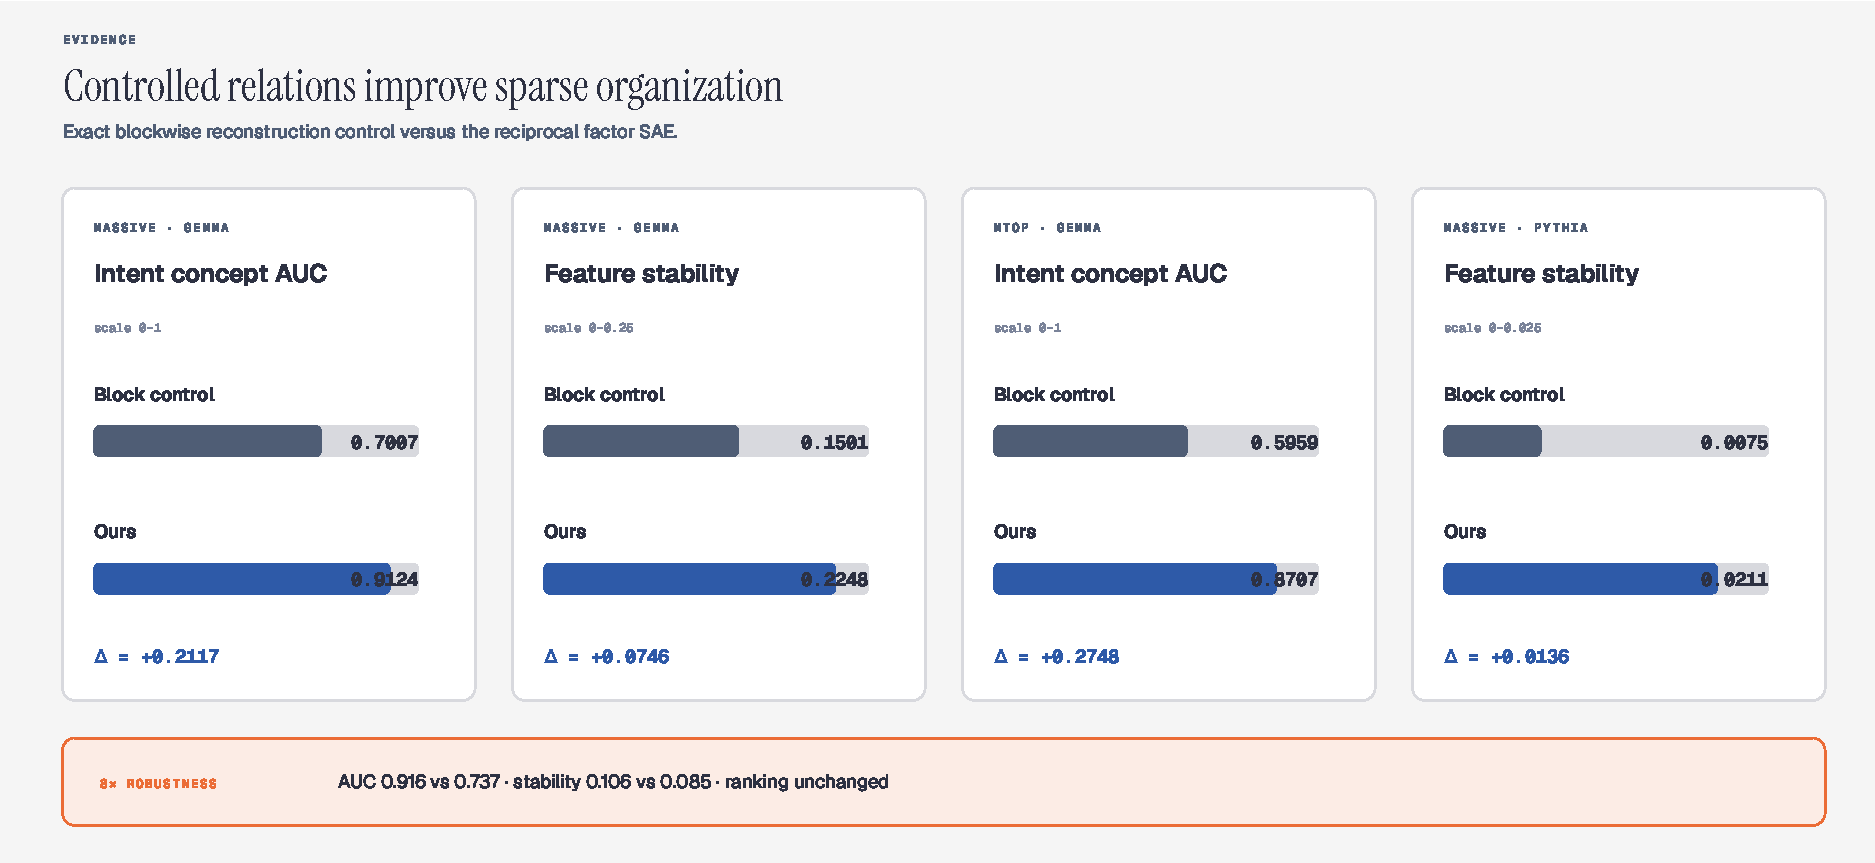
\includegraphics[width=\textwidth]{Figures/factor_sae_figure2_evidence.pdf}
\caption{The controlled-relation advantage transfers across datasets and model families and persists at eightfold width. All panels compare against the exact blockwise reconstruction control; the Pythia table and complete protocol are in Appendix~\ref{app:transfer-tables}.}
\label{fig:factor-sae-evidence}
\end{figure*}

The controlled-relation advantage persists when the dictionary is widened, exact translation IDs are removed, or the activation model is changed. Figure~\ref{fig:factor-sae-evidence} summarizes these three tests; the tables below and Appendix~\ref{app:transfer-tables} give the full results.

\begin{table*}[t]
\centering
\caption{MASSIVE width robustness. Dictionary width and activity double together from $4\times$/$L_0=64$ to $8\times$/$L_0=128$.}
\label{tab:factor-sae-width}
\resizebox{.94\textwidth}{!}{%
\begin{tabular}{llrrrrrr}
\toprule
Width & Method & AUC $\uparrow$ & Stability $\uparrow$ & Locale probe $\downarrow$ & Intent frac. $\uparrow$ & Locale frac. $\downarrow$ & FVE $\uparrow$ \\
\midrule
$4\times$ & Global BatchTopK & .7940 & .1278 & .9871 & .4579 & .4723 & .6618 \\
$4\times$ & Blockwise control & .7007 & .1501 & .9665 & .4830 & .4465 & .6627 \\
$4\times$ & \textbf{Ours} & \textbf{.9124} & \textbf{.2248} & \textbf{.8944} & \textbf{.7864} & \textbf{.1646} & .6098 \\
\midrule
$8\times$ & Global BatchTopK & .8094 & .0797 & .9908 & .4408 & .4637 & .7152 \\
$8\times$ & Blockwise control & .7373 & .0847 & .9760 & .4494 & .4562 & .7154 \\
$8\times$ & \textbf{Ours} & \textbf{.9156} & \textbf{.1063} & \textbf{.9397} & \textbf{.6708} & \textbf{.2530} & .6705 \\
\bottomrule
\end{tabular}%
}
\end{table*}

Doubling dictionary width and activity preserves the main ordering. At eightfold width, reciprocal supervision improves AUC by .1783 and stability by 25.6\% over the exact control. FVE remains within 6.3\% of the control, and intent AUC is nearly unchanged across widths (.9124 and .9156).

\begin{table*}[t]
\centering
\caption{MTOP transfer to held-out Hindi and Thai (three paired seeds). Lower language probe and $z_S$ intent are better.}
\label{tab:factor-sae-mtop}
\resizebox{\textwidth}{!}{%
\begin{tabular}{lrrrrrrr}
\toprule
Method & AUC $\uparrow$ & Stability $\uparrow$ & Margin $\uparrow$ & Lang. probe $\downarrow$ & R@1 $\uparrow$ & $z_S$ lang. $\uparrow$ & $z_S$ intent $\downarrow$ \\
\midrule
Raw $H$ & .7859 & .5443 & -.0724 & 1.0000 & .7998 & -- & -- \\
Global BatchTopK & $.6529\pm.0038$ & $.3605\pm.0023$ & $.0341\pm.0024$ & $.9837\pm.0020$ & $.7010\pm.0062$ & -- & -- \\
Blockwise control & $.5959\pm.0186$ & $.3701\pm.0119$ & $.0228\pm.0100$ & $.9416\pm.0050$ & $.4900\pm.0391$ & $.9795\pm.0027$ & $.5071\pm.0140$ \\
\textbf{Ours} & $\mathbf{.8707\pm.0017}$ & $\mathbf{.4978\pm.0153}$ & $\mathbf{.3441\pm.0105}$ & $\mathbf{.9278\pm.0034}$ & $\mathbf{.7809\pm.0166}$ & $\mathbf{.9857\pm.0035}$ & $\mathbf{.4639\pm.0062}$ \\
\bottomrule
\end{tabular}%
}
\end{table*}

MTOP tests whether exact translations are necessary. Training uses German, English, Spanish, and French, while Hindi and Thai are held out. Because MTOP has no parallel semantic IDs, stability compares each feature's 50-intent activation profile across the two test languages. Reciprocal supervision improves AUC by .2748, stability by .1277, relation margin by .3214, and retrieval R@1 by .2910 over the exact blockwise control. The same objective therefore transfers without exact translations or dataset-specific architectural changes.

Pythia-160M tests a different activation geometry. Reciprocal supervision raises stability from .0075 to .0211 and improves relation margin by .4797 over the blockwise control, with the same direction in all three paired seeds. It also improves feature orientation, locale leakage, and the opposing route. The absolute AUC change is small in this weaker activation space; stability, margin, and route organization provide the transfer evidence. No Pythia-specific loss or sparsity setting is introduced.

The component ablations support reciprocal binary supervision. One-sided training attains slightly higher intent AUC (.9165 versus .9124), but reciprocal training improves stability by .0434, raises the intent-oriented fraction by .0941, lowers the locale-oriented fraction by .0781, and reduces $z_S$ intent leakage by .0787. The triplet loss retains more reconstruction FVE (.6427 versus .6098) but is lower on AUC, stability, locale leakage, and feature orientation. These results motivate the reciprocal binary objective used throughout the transfer experiments.
